\documentclass[12pt,a4paper]{article}
\usepackage[utf8]{inputenc}
\usepackage[margin=2.5cm]{geometry}
\usepackage{amsmath}
\usepackage{amsfonts}
\usepackage{amssymb}
\usepackage{graphicx}
\usepackage{float}
\usepackage{booktabs}
\usepackage{array}
\usepackage{multirow}
\usepackage{url}
\usepackage{hyperref}
\usepackage{siunitx}
\usepackage{caption}
\usepackage{subcaption}

% Configure hyperref
\hypersetup{
    colorlinks=true,
    linkcolor=black,
    filecolor=magenta,      
    urlcolor=blue,
    citecolor=black,
}

% Configure siunitx for proper unit formatting
\sisetup{
    separate-uncertainty = true,
    multi-part-units = repeat
}

\title{\textbf{Chamber Pressure and Specific Impulse of a Rocket Engine}}
\author{Tjark Osterloh}
\date{May 27, 2025}

\begin{document}

\maketitle

\section{Introduction}

When designing a rocket, the rocket engine will be a crucial component. If you choose not to buy an already existing engine, but decide to design your own, you will see that having an efficient engine will be one of your big priorities. Your rocket airframe might be the most aerodynamic, and your aviation controls are perfect, but it would not matter if your engine cannot compulse it through space, because your engine works inefficiently.

I have come to find this exact problem when as a hobbyist trying to design a rocket and my own liquid fueled rocket engine, getting an efficient rocket engine is crucial. And efficiency in such will often be measured in specific impulse. Now there are alot of things impacting specific impulse which have to be considered when designing an engine. I found that some of them like ambient pressure are constrained anyways so I won't be able to impact them to make my engine more efficient. Others like the fuel choice are often very heavily researched already and have a simple answer, where using hydrogen with oxygen will give a higher specific impulse then kerosine with nitrous oxide.

But one of the factors which I find hard to follow, is the impact of chamber pressure of a rocket, so the pressure inside the engine before the fuel leaves through the nozzle on specific impulse. Not Knowing what pressure should be inside the engine has haltet my design lately, because the chamber pressure also affects the nozzle ratios and so on... . Through my research I have found numerous nasa articles about optimal chamber pressure, but I haven't been able to visualize the impact or if there is really any myself.

This is why in my IA I will investigate in isolation the impact of chamber pressure on specific impulse.

\section{Research Question}

What is the impact of air chamber pressure inside a small plastic water bottle as a rocket engine on specific impulse?

\section{Background Information}

\subsection{Chamber Pressure}

Chamber pressure is very important in rocketry, and rocket propulsion, the pressure inside the engines chamber will decide how strong the exhaust gases are pushed out. Chamber pressure relates to thermodynamics, fluid dynamics and Newton's 3rd law in physics \cite{ref2}. Chamber pressure is important beyond rocketry, it is important in internal combustion engines, and jet propulsion. Higher pressure gases affect how the rocket engine functions \cite{ref1}. 

\begin{equation}
W = P\Delta V
\end{equation}

Higher pressures expect more work. The chamber pressures of the Saturn V's (the rocket which flew to the moon) rocket engines was around \SI{7}{\mega\pascal}, whilst the pressure inside the Raptor engines (propelling space x's star ship) is \SI{35}{\mega\pascal} significantly higher.

\subsection{Impulse}

Impulse is a measure of the total momentum change something has, in rockets it would be the momentum a rocket engine delivers to start moving \cite{ref5}. 

\begin{equation}
J = F\Delta T
\end{equation}

Impulse is very important in reference to change in momentum and energy. Impulse is very important in aerospace engineering and spacecraft design, to work on efficiency \cite{ref3}. To have high impulse means that the rocket is stronger which is often seen positive, impulse iis also dependent on the time the force is applied \cite{ref4}, but the saturn v engine produced \SI{6770}{\kilo\newton} of thrust at sea level, whilst the raptor engine only produces \SI{2260}{\kilo\newton} of thrust at sea level. This decrease could be due to the higher pressure, but is likely just because a single Saturn V engine was expected to be stronger than one Raptor engine.

\subsection{Mass Flow Rate}

Mass flow rate is required for specific impulse, it is not part of the ib syllabus but it is a great measure of how much propellant is exerted from an engine. It ties into fluid dynamics \cite{ref6}, higher mass flow rate means there are more gases exerted in less time. It is very important for any kind of fuel engine, because it gives an estimate of how much fuel is required for the engine \cite{ref7}. Mass flow rate is affected by the viscosity of the liquid, the mass of the liquid, and the area which the mass flows through, in the ocean there is more movement then in a lake.

\subsection{Specific Impulse}

Specific impulse is a measurement of fuel efficiency, high specific impulse means the rocket is highly efficient, defined as the amount of thrust produced per unit of propellant consumed over time. Essentially, it tells us how effectively a rocket engine uses fuel. The higher the specific impulse, the more efficient the engine is, meaning it can produce more thrust while using less fuel. Expressed in seconds.

Specific impulse is often affected by the propellant type, what kind of fuel is used in a rocket impacts its efficiency. The engine design is also very important, the size and ratio of the combustion chamber and the ratio to the nozzle affect how efficient the engine will function. The velocity at which the gases exit the nozzle also affect the specific impulse. The temperature of the combustion affects the specific impulse, higher temperatures often lead to higher efficiency \cite{ref9}. And the mass of the exhaust gases also impact the engine efficiency, often lighter particles will be more efficient.

The ambient pressure is also very important, bigger pressure differentials can affect the exhaust flow, so in a vacuum the difference would be infinite, whilst on sea level the ambient pressure is high already. I am investigating this statement, because by increasing the chamber pressure, I will increase the diffrence from chamber pressure to atmospheric pressure.

The specific impulse of a saturn v engine was \SI{263}{\second} whilst a raptor engine had one of \SI{327}{\second}, both at sea level \cite{ref8}. Now i hope the increase in efficiency is due to the higher chamber pressure, but the saturn v used less efficient kerosine as a fuel then the methane used by space x, and the velocity of the exhaust gases from the raptor are also higher, and the engine design used by the saturn as a whole was less efficient using a gas generator cycle, instead of a full flow stage cycle.

\subsection{Nozzle Shape}

Nozzle shape of a rocket engine is very important, the width/size/curvature of a nozzle will determine how much fuel can be expelled by limiting it, it also determines what kind of chamber pressures a rocket engine can function in \cite{ref10}. to be expected is that small nozzle sizes will cause higher pressures in an open system, as the gases need to compress to fit through the nozzle. There is a lot of research into nozzle shapes where typically converging diverging nozzles are overall the best, gases are accelerated in the converging part and after reaching mach 1 they get accelerated even more in the diverging part \cite{ref11}. This is very interesting, but in this experiment the nozzle will just be a small hole at the end of a valve. It is important though that it is small, because this might limit the mass flow rate.

\subsection{Rocketry}

Rocket engines rely significantly on those kinds of variables to reach efficiency. Rocket engines and engines of all kinds are often very inefficient, so the importance of efficiency is highlighted once more \cite{ref12,ref13}. Rocketry is very important to us humans in fields like safety but also and more interesting space exploration and fast travel.

\section{Hypothesis}

I am predicting that there will be some kind of proportional behaviour between the chamber pressure of a rocket and the impulse of the rocket. Furthermore I will predict that in moderate pressures (all the pressures that I hope to test), the higher pressure will have a linear correlation with higher specific impulse.

I believe this because of the following correlations which i have found:

\begin{align}
W &\propto P \\
W &\propto F \\
F &\propto J \\
\therefore P &\propto J
\end{align}

Now considering that the specific impulse can be derived from impulse i predict that higher pressure will also cause more efficient engine. Although higher pressure resulting in efficiency might sound unintuitive as high pressures sound very violent.

Nevertheless I predict a linear direct correlation, which does not converge at all (definitely not in the range of pressures in my experiment).

\section{Variables}

\begin{table}[H]
\centering
\caption{Variables in the experiment}
\begin{tabular}{@{}lp{10cm}@{}}
\toprule
\textbf{Type} & \textbf{Variables} \\
\midrule
Independent & Number of pumps / chamber pressure \\
\midrule
\multirow{5}{*}{Dependent} & Force exerted \\
& Time taken to exert \\
& Impulse \\
& Mass flow rate \\
& Specific impulse \\
\midrule
\multirow{3}{*}{Control} & Volume of rocket, for consistency and no interference in $PV=nRT$ \\
& Positioning on the force plate, for equal measurements \\
& Temperature, for consistency and no interference in $PV=nRT$ \\
\bottomrule
\end{tabular}
\end{table}

\section{Methodology}

\subsection{Materials}
\begin{itemize}
\item Water rocket setup (little plastic water bottle, a pump, a valve, a stand, o rings)
\item Air
\item Force measuring plate
\item Water
\item Measuring cylinder
\item \SI{320}{\gram} of rocks
\end{itemize}

\begin{figure}[H]
\centering
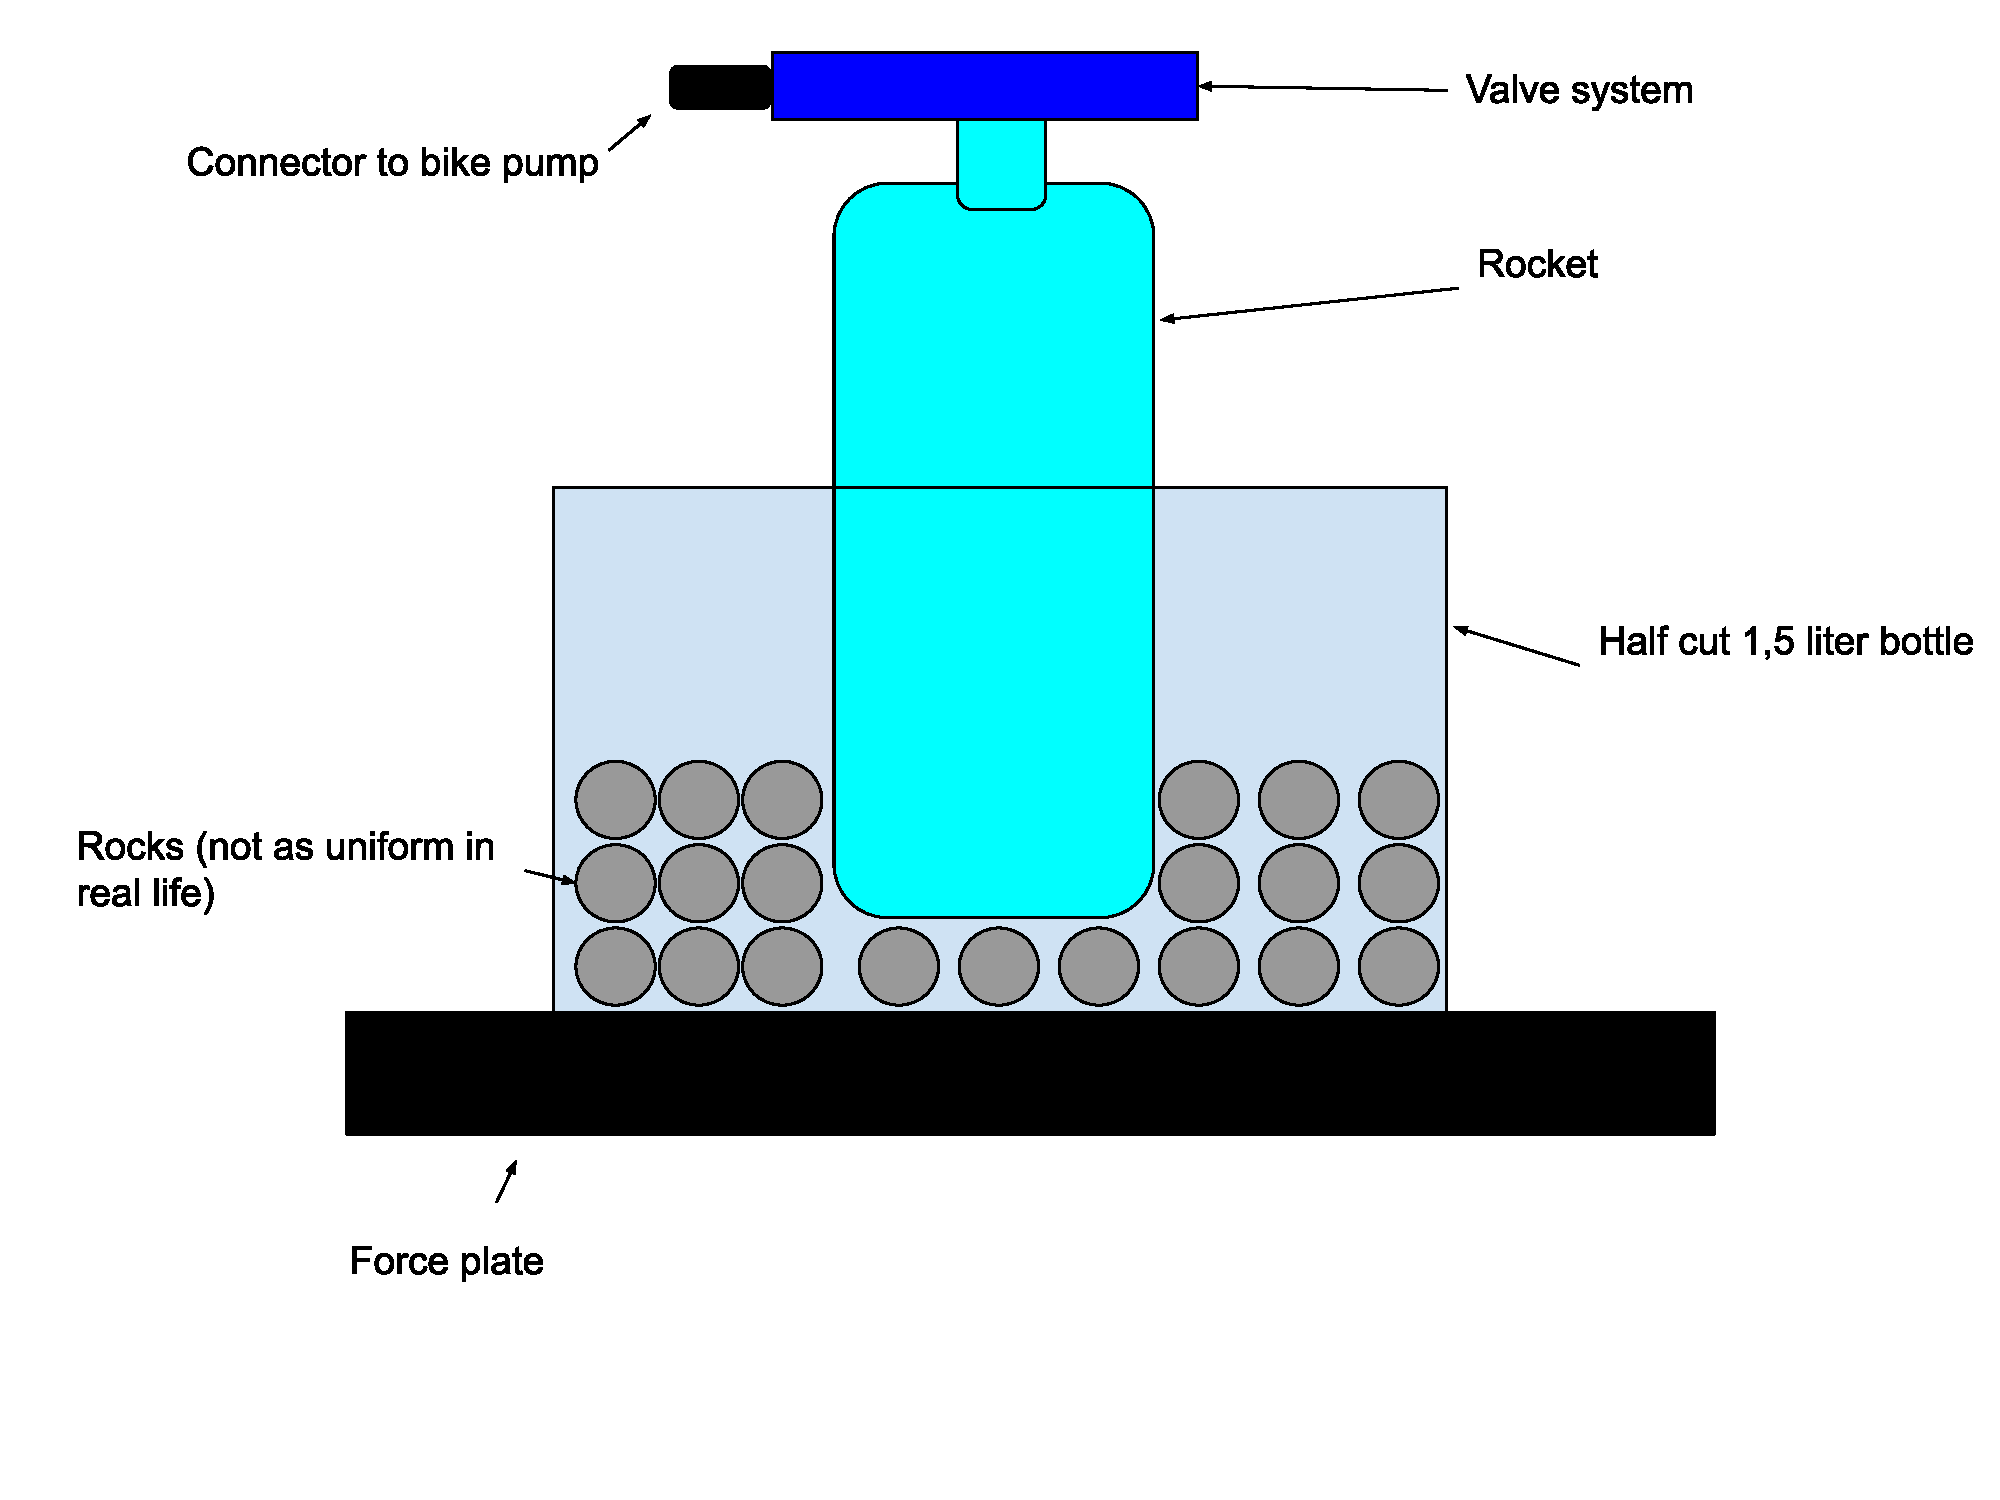
\includegraphics[width=0.8\textwidth]{measuring force.pdf}
\caption{Force measurement setup}
\label{fig:measuring_force}
\end{figure}

\subsection{Procedure}

\subsubsection{Preparation \& Setup}
\begin{enumerate}
\item Cut a \SI{2.5}{\liter} cola bottle in half.
\item Fill the bottom half with \SI{20}{\gram} of rocks.
\item Place the bottle/rocket in the half lower half of the cola bottle, positioning it securely.
\item Surround the rocket base with \SI{300}{\gram} of rocks to prevent movement
\end{enumerate}

\subsubsection{Force Plate Setup \& Air Pressure Control}
\begin{enumerate}
\item Position the cola bottle on the force plate, ensuring stability.
\item Mark the exact location of the bottle on the force plate.
\item Tare the force plate to reset baseline measurement.
\item Ensure the system is airtight before pressurization.
\end{enumerate}

\subsubsection{Pressurization \& Measurement Process}
\begin{enumerate}
\item Begin pressurizing the rocket, at 10, 20, 30, 40, 50 pumps.
\item Start the force plate measurement.
\item Open the bottle valve to release pressure.
\item Record the force plate readings throughout the process.
\item Repeat the procedure with different pressure levels for comparison.
\end{enumerate}

\subsection{Risk Assessment}

\begin{table}[H]
\centering
\caption{Risk assessment}
\begin{tabular}{@{}p{4cm}p{6cm}p{6cm}@{}}
\toprule
\textbf{Risk factor} & \textbf{Description} & \textbf{Safety measure} \\
\midrule
High pressure water bottle & The experiment requires high pressure, at such pressure the bottle might explode & Test pressures much higher than the experiment will be conducted at, if the rocket survives, it will also at the pressures that are investigated \\
\bottomrule
\end{tabular}
\end{table}

\section{Data Collection}

\subsection{Raw Data}

From my collected data I will show by the use of the example of 50 pumps all my calculations:

First, using the number of Pumps as an independent variable did not satisfy me, instead I measured the volume of the rocket by filling it up with water.

$V_{\text{rocket}} = \SI{250 \pm 1}{\milli\liter}$

Also the volume added to every pump, by measuring the displacement of air by pumping air into a cylinder filled with water.

See Figure \ref{fig:water_displacement} for visual comparison of the water displacement measurement.

\begin{figure}[H]
\centering
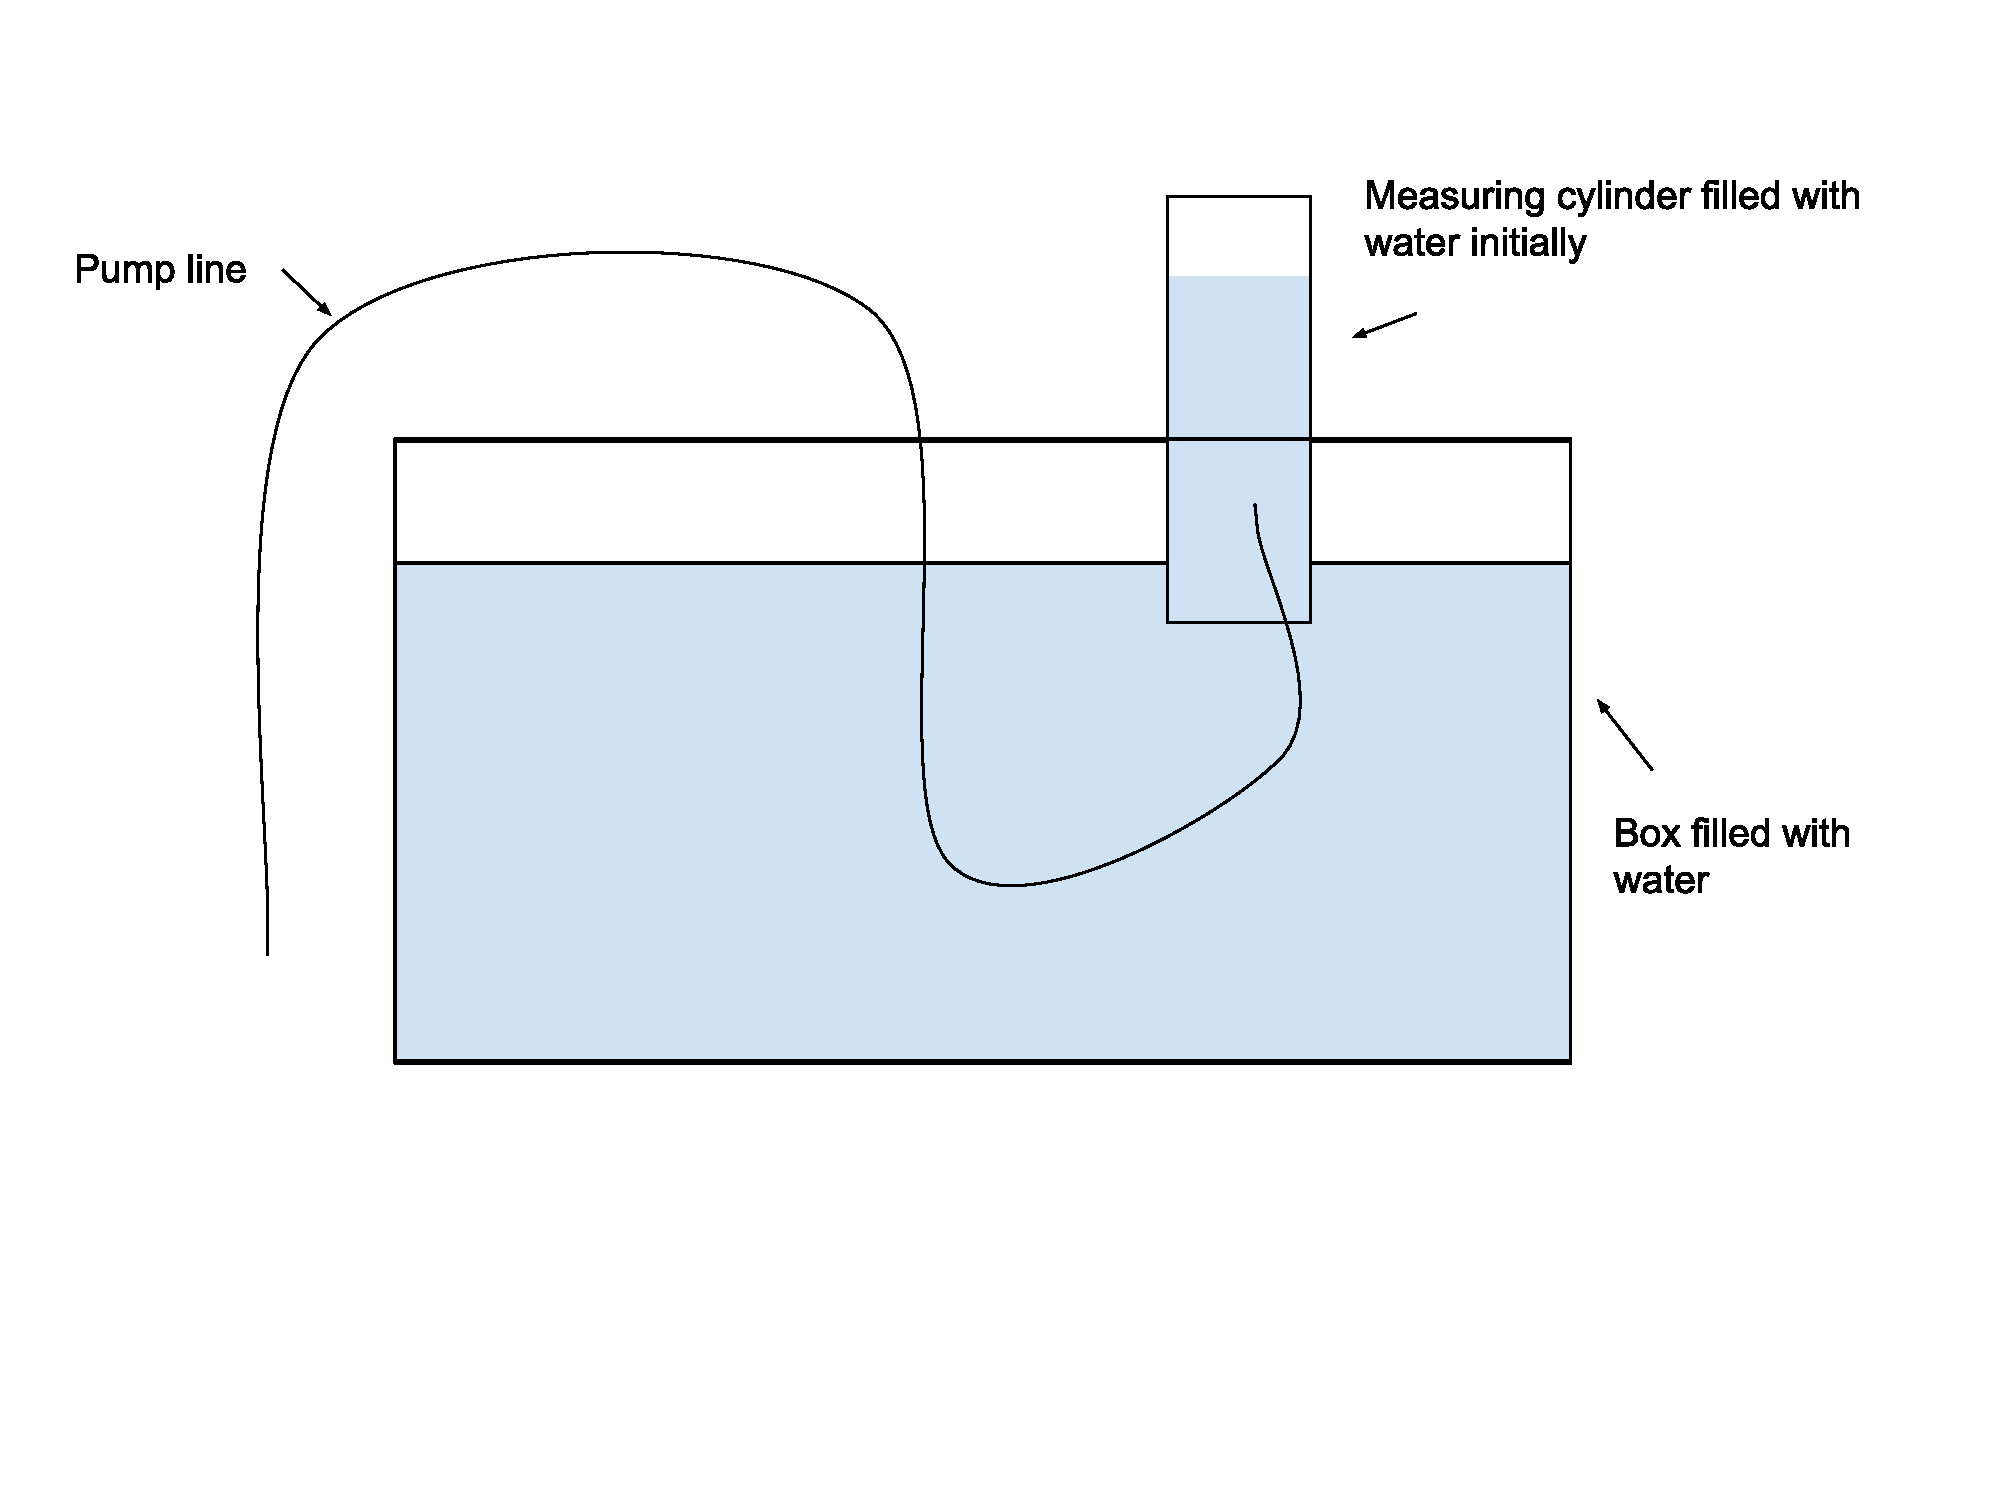
\includegraphics[width=0.8\textwidth]{measuring the water displacement.pdf}
\caption{Water displacement measurement}
\label{fig:water_displacement}
\end{figure}

\begin{align}
V_{\text{per pump}} &= V_{\text{final measurement}} - V_{\text{initial measurement}} \\
&= \SI{47.0 \pm 0.5}{\milli\liter} - \SI{9.0 \pm 0.5}{\milli\liter} \\
&= \SI{38 \pm 1}{\milli\liter}
\end{align}

\begin{align}
V_{50} &= V_{\text{rocket}} + 50 \times V_{\text{per pump}} \\
&= \SI{250 \pm 1}{\milli\liter} + \SI{38 \pm 1}{\milli\liter} \times 50 \\
&= \SI{2150 \pm 51}{\milli\liter}
\end{align}

Now I tried finding the amount of moles after 50 pumps.

\begin{equation}
n_{50} = n_{\text{rocket}} \text{ (250 ml of air)} + 50 \times n_{\text{per pump}} \text{ (38 ml of air)}
\end{equation}

I measured the temperature at the start of the experiment and at the end.

\begin{align}
T_1 &= \SI{23.1 \pm 0.1}{\celsius} \\
\end{align}
\begin{align}
T_2 &= \SI{23.5 \pm 0.1}{\celsius} \\
\end{align}
\begin{align} T_{\text{avg}} &= \frac{23.1 + 23.5}{2} \\
&= \SI{23.3}{\celsius}
\end{align}

I was unable to measure the density of my local air, but through research \cite{ref14}. I found the expected $M_r$ for my pressure and Temperature, assuming it is constant. I treated researched values as constant and assumed no uncertainties.

$M_{r,\text{air}} = \SI{0.0290}{\kilo\gram\per\mol}$

Now assuming the ideal gas law:

\begin{equation}
PV = nRT
\end{equation}

I could calculate the pressure, from the initial pressure, i could not measure my local atmospheric pressure, but in my weather app i found the local pressure at the time of my experiment, see appendix.

\begin{align}
n &= \frac{PV}{RT} \\
n_{\text{rocket}} &= \frac{\SI{1.016e5}{\pascal} \times \SI{0.000250 \pm 0.000001}{\meter\cubed}}{\SI{8.31}{\joule\per\mol\per\kelvin} \times \SI{296.3 \pm 0.1}{\kelvin}} = \SI{0.01031}{\mol} \\
n_{\text{Pump}} &= \frac{\SI{1.016e5}{\pascal} \times \SI{0.000038}{\meter\cubed}}{\SI{8.31}{\joule\per\mol\per\kelvin} \times \SI{296.3 \pm 0.1}{\kelvin}} = \SI{0.001567}{\mol} \\
n_{50} &= \SI{0.010310}{\mol} + 50 \times \SI{0.001567}{\mol} = \SI{0.08866}{\mol}
\end{align}

Assuming temp is constant

$P_{\text{atm}} \propto \frac{R}{V}$, $\SI{1.016e5}{} \propto \frac{\SI{0.01031}{\mol}}{\SI{0.000250 \pm 0.000001}{\meter\cubed}}$

\begin{align}
P_{50} &= P_1 \times \frac{R}{V} \\
&= \SI{1.016e5}{\pascal} \times \frac{\SI{0.08866}{\mol} / \SI{0.000250 \pm 0.000001}{\meter\cubed}}{\SI{0.01031}{\mol} / \SI{0.000250 \pm 0.000001}{\meter\cubed}} \\
&= \SI{8.737e5}{\pascal}
\end{align}

But actually

$\frac{V_{50}}{V_{\text{rocket}}} \propto \frac{n_{50}}{n_{\text{rocket}}}$

So

\begin{align}
P_{50} &= P_{\text{atm}} \times \frac{V_{50}}{V_{\text{rocket}}} \\
&= \SI{1.016e5}{\pascal} \times \frac{\SI{0.002150 \pm 0.000051}{\meter\cubed}}{\SI{0.000250 \pm 0.000001}{\meter\cubed}} \\
&= \SI{8.737e5}{\pascal}
\end{align}

$\%\text{uncertainty}(P_{50}) = \left(\frac{\pm \SI{1}{\milli\liter}}{\SI{250}{\milli\liter}} + \frac{\pm \SI{51}{\milli\liter}}{(\SI{2150}{\milli\liter} - \SI{250}{\milli\liter})}\right) \times 100 = 3.08\%$

Now that I have pressure as my independent variable, I can calculate the impulse. From my measurements I got the time where the peak measurement in the force plate starts and ends so first I took averages of change in time and peak force.

For 50 pump measurements:

\begin{align}
F_{\text{avg peak 50}} &= \frac{F_1 + F_2 + F_3 + F_4 + F_5}{5} \\
&= \frac{\SI{32 \pm 1}{\newton} + \SI{34 \pm 1}{\newton} + \SI{19 \pm 1}{\newton} + \SI{22 \pm 1}{\newton} + \SI{30 \pm 1}{\newton}}{5} \\
&= \SI{27.4 \pm 1}{\newton}
\end{align}

\begin{align}
\Delta t_{\text{avg 50}} &= \frac{(T_2 - T_1 + T_4 - T_3 + T_6 - T_5 + T_8 - T_7 + T_{10} - T_9)}{5} \\
&= \frac{(\SI{3087.6 \pm 0.1}{\milli\second} - \SI{3029.8 \pm 0.1}{\milli\second} + \SI{2202.0 \pm 0.1}{\milli\second} - \SI{2192.8 \pm 0.1}{\milli\second} + \ldots)}{5} \\
&= \SI{39.82 \pm 0.2}{\milli\second} \\
&= \SI{0.03982 \pm 0.0002}{\second}
\end{align}

Now because the graph was in a shape of a triangle i could use the formula for the area of a triangle to calculate impulse

\begin{align}
J_{50} &= A_t = \frac{1}{2}(b\Delta t h F) \\
&= \frac{1}{2} \times (\SI{0.03982 \pm 0.0002}{\second} \times \SI{27.4 \pm 1}{\newton}) \\
&= \SI{0.546}{\newton\second}
\end{align}

$\%\text{uncertainty}(J_{50}) = \left(\frac{\pm \SI{0.0002}{\second}}{\SI{0.03982}{\second}} + \frac{\pm \SI{1}{\newton}}{\SI{27.4}{\newton}}\right) \times 100 = 4.15\%$

Now that I know what the change in momentum is, now i can find what mass carries this momentum out, the mass flow rate.

$\dot{m} = \frac{\Delta m}{\Delta t}$

I dont have the mass of the air, but from my previous research i can figure out the density of air

\begin{align}
N &= \frac{m}{M_r} \\
\rho &= \frac{m}{V} \\
PV &= nRT = \frac{mRT}{M_r}, \quad P = \frac{\rho RT}{M_r}, \quad \rho = \frac{PM_r}{RT}
\end{align}

\begin{align}
\rho_{\text{atm}} &= \frac{P_{\text{atm}} \times M_{r,\text{air}}}{R \times T} \\
&= \frac{\SI{1.016e5}{\pascal} \times \SI{0.0290}{\kilo\gram\per\mol}}{\SI{8.31}{\joule\per\mol\per\kelvin} \times \SI{296.3}{\kelvin}} \\
&= \SI{1.195}{\kilo\gram\per\meter\cubed}
\end{align}

I also researched what density air should be at \SI{23}{\celsius} and standard pressure. I was unable to find data specific for \SI{23.2}{\celsius} and my specific pressure. But for \SI{23}{\celsius} and standard pressure were $\rho = \SI{1.289}{\kilo\gram\per\meter\cubed}$, so my calculation was probably not far off.

\begin{align}
\rho_{50} &= \frac{P_{50} \times M_{r,\text{air}}}{R \times T} \\
&= \frac{\SI{8.737e5}{\pascal} \times \SI{0.0290}{\kilo\gram\per\mol}}{\SI{8.31}{\joule\per\mol\per\kelvin} \times \SI{296.3}{\kelvin}} \\
&= \SI{10.29}{\kilo\gram\per\meter\cubed}
\end{align}
\begin{align}
m_i &= \SI{1.195}{\kilo\gram\per\meter\cubed} \times \SI{0.000250 \pm 0.000001}{\meter\cubed} \\
&= \SI{0.0003}{\kilo\gram} \\
m_{50} &= \SI{10.29}{\kilo\gram\per\meter\cubed} \times \SI{0.000250 \pm 0.000001}{\meter\cubed} \\
&= \SI{0.002571}{\kilo\gram}
\end{align}

\begin{align}
\dot{m}_{50} &= \frac{\Delta m}{\Delta t} \\
&= \frac{\SI{0.002571}{\kilo\gram} - \SI{0.0003}{\kilo\gram}}{\SI{0.03982}{\second}} \\
&= \SI{0.0570}{\kilo\gram\per\second}
\end{align}

And because i only consider the change in mass and temp is constant i don't need to consider its uncertainty

\begin{align}
\%\text{uncertainty}(\dot{m}_{50}) &= 3.08\% + 0.4\% + \frac{\pm \SI{2}{\milli\liter}}{\SI{250}{\milli\liter}} \times 100 \\
&= 4.28\%
\end{align}

With the mass flow rate we can finally calculate the efficiency of the rocket dependent on the pressure, the specific impulse.

\begin{equation}
I_{sp} = \frac{F}{\dot{m} \times g}
\end{equation}

This required the average force, for a triangle

\begin{equation}
F_{\text{avg}} = H_{\text{avg}} = \frac{2A}{\text{Base}(\Delta T)}
\end{equation}

And i researched the gravitational acceleration of my location\cite{ref1}5. .

\begin{align}
I_{sp50} &= \frac{2 \times J_{50}}{\Delta t \times \dot{m}_{50} \times g} \\
&= \frac{2 \times \SI{0.546}{\newton\second}}{\SI{0.03982}{\second} \times \SI{0.0570}{\kilo\gram\per\second} \times \SI{9.818}{\meter\per\second\squared}} \\
&= \SI{48.9}{\second}
\end{align}

\begin{align}
\%\text{uncertainty}(I_{sp50}) &= 4.56\% \times 2 + \frac{\pm \SI{0.0002}{\second}}{\SI{0.03982}{\second}} + 4.28\% \\
&= 13.09\%
\end{align}

\subsection{Tables}

\begin{table}[H]
\centering
\caption{Pressure and volume data for different pump amounts}
\begin{tabular}{@{}cccc@{}}
\toprule
\textbf{Amount of pumps} & \textbf{Volume / $\pm$\SI{0.000002}{\meter\cubed}} & \textbf{Pressure / \si{\pascal}} & \textbf{Relative uncertainty} \\
\midrule
0 & 0.000250 & \num{1.016e5} & 0.40\% \\
10 & 0.000630 & \num{2.560e5} & 3.29\% \\
20 & 0.001010 & \num{4.105e5} & 3.16\% \\
30 & 0.001390 & \num{5.649e5} & 3.12\% \\
40 & 0.001770 & \num{7.193e5} & 3.10\% \\
50 & 0.002150 & \num{8.738e5} & 3.08\% \\
\bottomrule
\end{tabular}
\end{table}

\begin{table}[H]
\centering
\caption{Force measurement data}
\begin{tabular}{@{}cccc@{}}
\toprule
\textbf{Pumps amount} & \textbf{Peak start / \si{\second} $\pm$ 0.0001} & \textbf{Peak end / \si{\second} $\pm$ 0.0001} & \textbf{Peak height / \si{\newton} $\pm$ 1} \\
\midrule
50 & 2.5071 & 2.5843 & 19 \\
40 & 4.8642 & 4.9227 & 12 \\
30 & 2.9819 & 3.0025 & 24 \\
20 & 2.1416 & 2.1864 & 12 \\
10 & 3.8678 & 3.8821 & 14 \\
50 & 2.3462 & 2.3567 & 34 \\
40 & 3.5060 & 3.5140 & 40 \\
30 & 1.8302 & 1.8381 & 27 \\
20 & 2.1203 & 2.1328 & 17 \\
10 & 2.3507 & 2.3630 & 17 \\
50 & 2.1928 & 2.2020 & 32 \\
40 & 2.0100 & 2.0240 & 26 \\
30 & 2.6686 & 2.6769 & 24 \\
20 & 1.9926 & 2.0040 & 20 \\
10 & 1.5973 & 1.6063 & 16 \\
50 & 3.0298 & 3.0876 & 22 \\
40 & 1.7300 & 1.7791 & 12 \\
30 & 4.0077 & 4.0268 & 20 \\
20 & 3.6033 & 3.6281 & 17 \\
10 & 2.1055 & 2.1473 & 4 \\
50 & 2.6245 & 2.6689 & 30 \\
40 & 2.6613 & 2.6804 & 19 \\
30 & 4.6452 & 4.6890 & 11 \\
20 & 2.0122 & 2.0399 & 14 \\
10 & 2.2739 & 2.2986 & 5 \\
\bottomrule
\end{tabular}
\end{table}

\begin{table}[H]
\centering
\caption{Average measurements and impulse calculations}
\begin{tabular}{@{}ccccc@{}}
\toprule
\textbf{Average} & \textbf{Change in time / \si{\second}} & \textbf{Peak height / \si{\newton}} & \textbf{Impulse} & \textbf{Uncertainty} \\
\midrule
50 & 0.0398 & 27 & 0.55 & 4.15\% \\
40 & 0.0297 & 22 & 0.32 & 5.26\% \\
30 & 0.0199 & 21 & 0.21 & 5.72\% \\
20 & 0.0242 & 16 & 0.19 & 7.08\% \\
10 & 0.0204 & 11 & 0.11 & 9.91\% \\
\bottomrule
\end{tabular}
\end{table}

\begin{table}[H]
\centering
\caption{Mass flow rate and specific impulse data}
\begin{tabular}{@{}ccccc@{}}
\toprule
\textbf{Pumps amount} & \textbf{Mass flow rate / \si{\kilo\gram\per\second}} & \textbf{Uncertainty} & \textbf{Specific impulse / \si{\second}} & \textbf{Uncertainty} \\
\midrule
10 & 0.0222 & 4.49\% & 51 & 25.29\% \\
20 & 0.0375 & 4.36\% & 43 & 19.34\% \\
30 & 0.0683 & 4.32\% & 32 & 16.76\% \\
40 & 0.0583 & 4.30\% & 38 & 15.49\% \\
50 & 0.0570 & 4.28\% & 49 & 13.09\% \\
\bottomrule
\end{tabular}
\end{table}

\subsection{Graphs}

\begin{figure}[H]
\centering
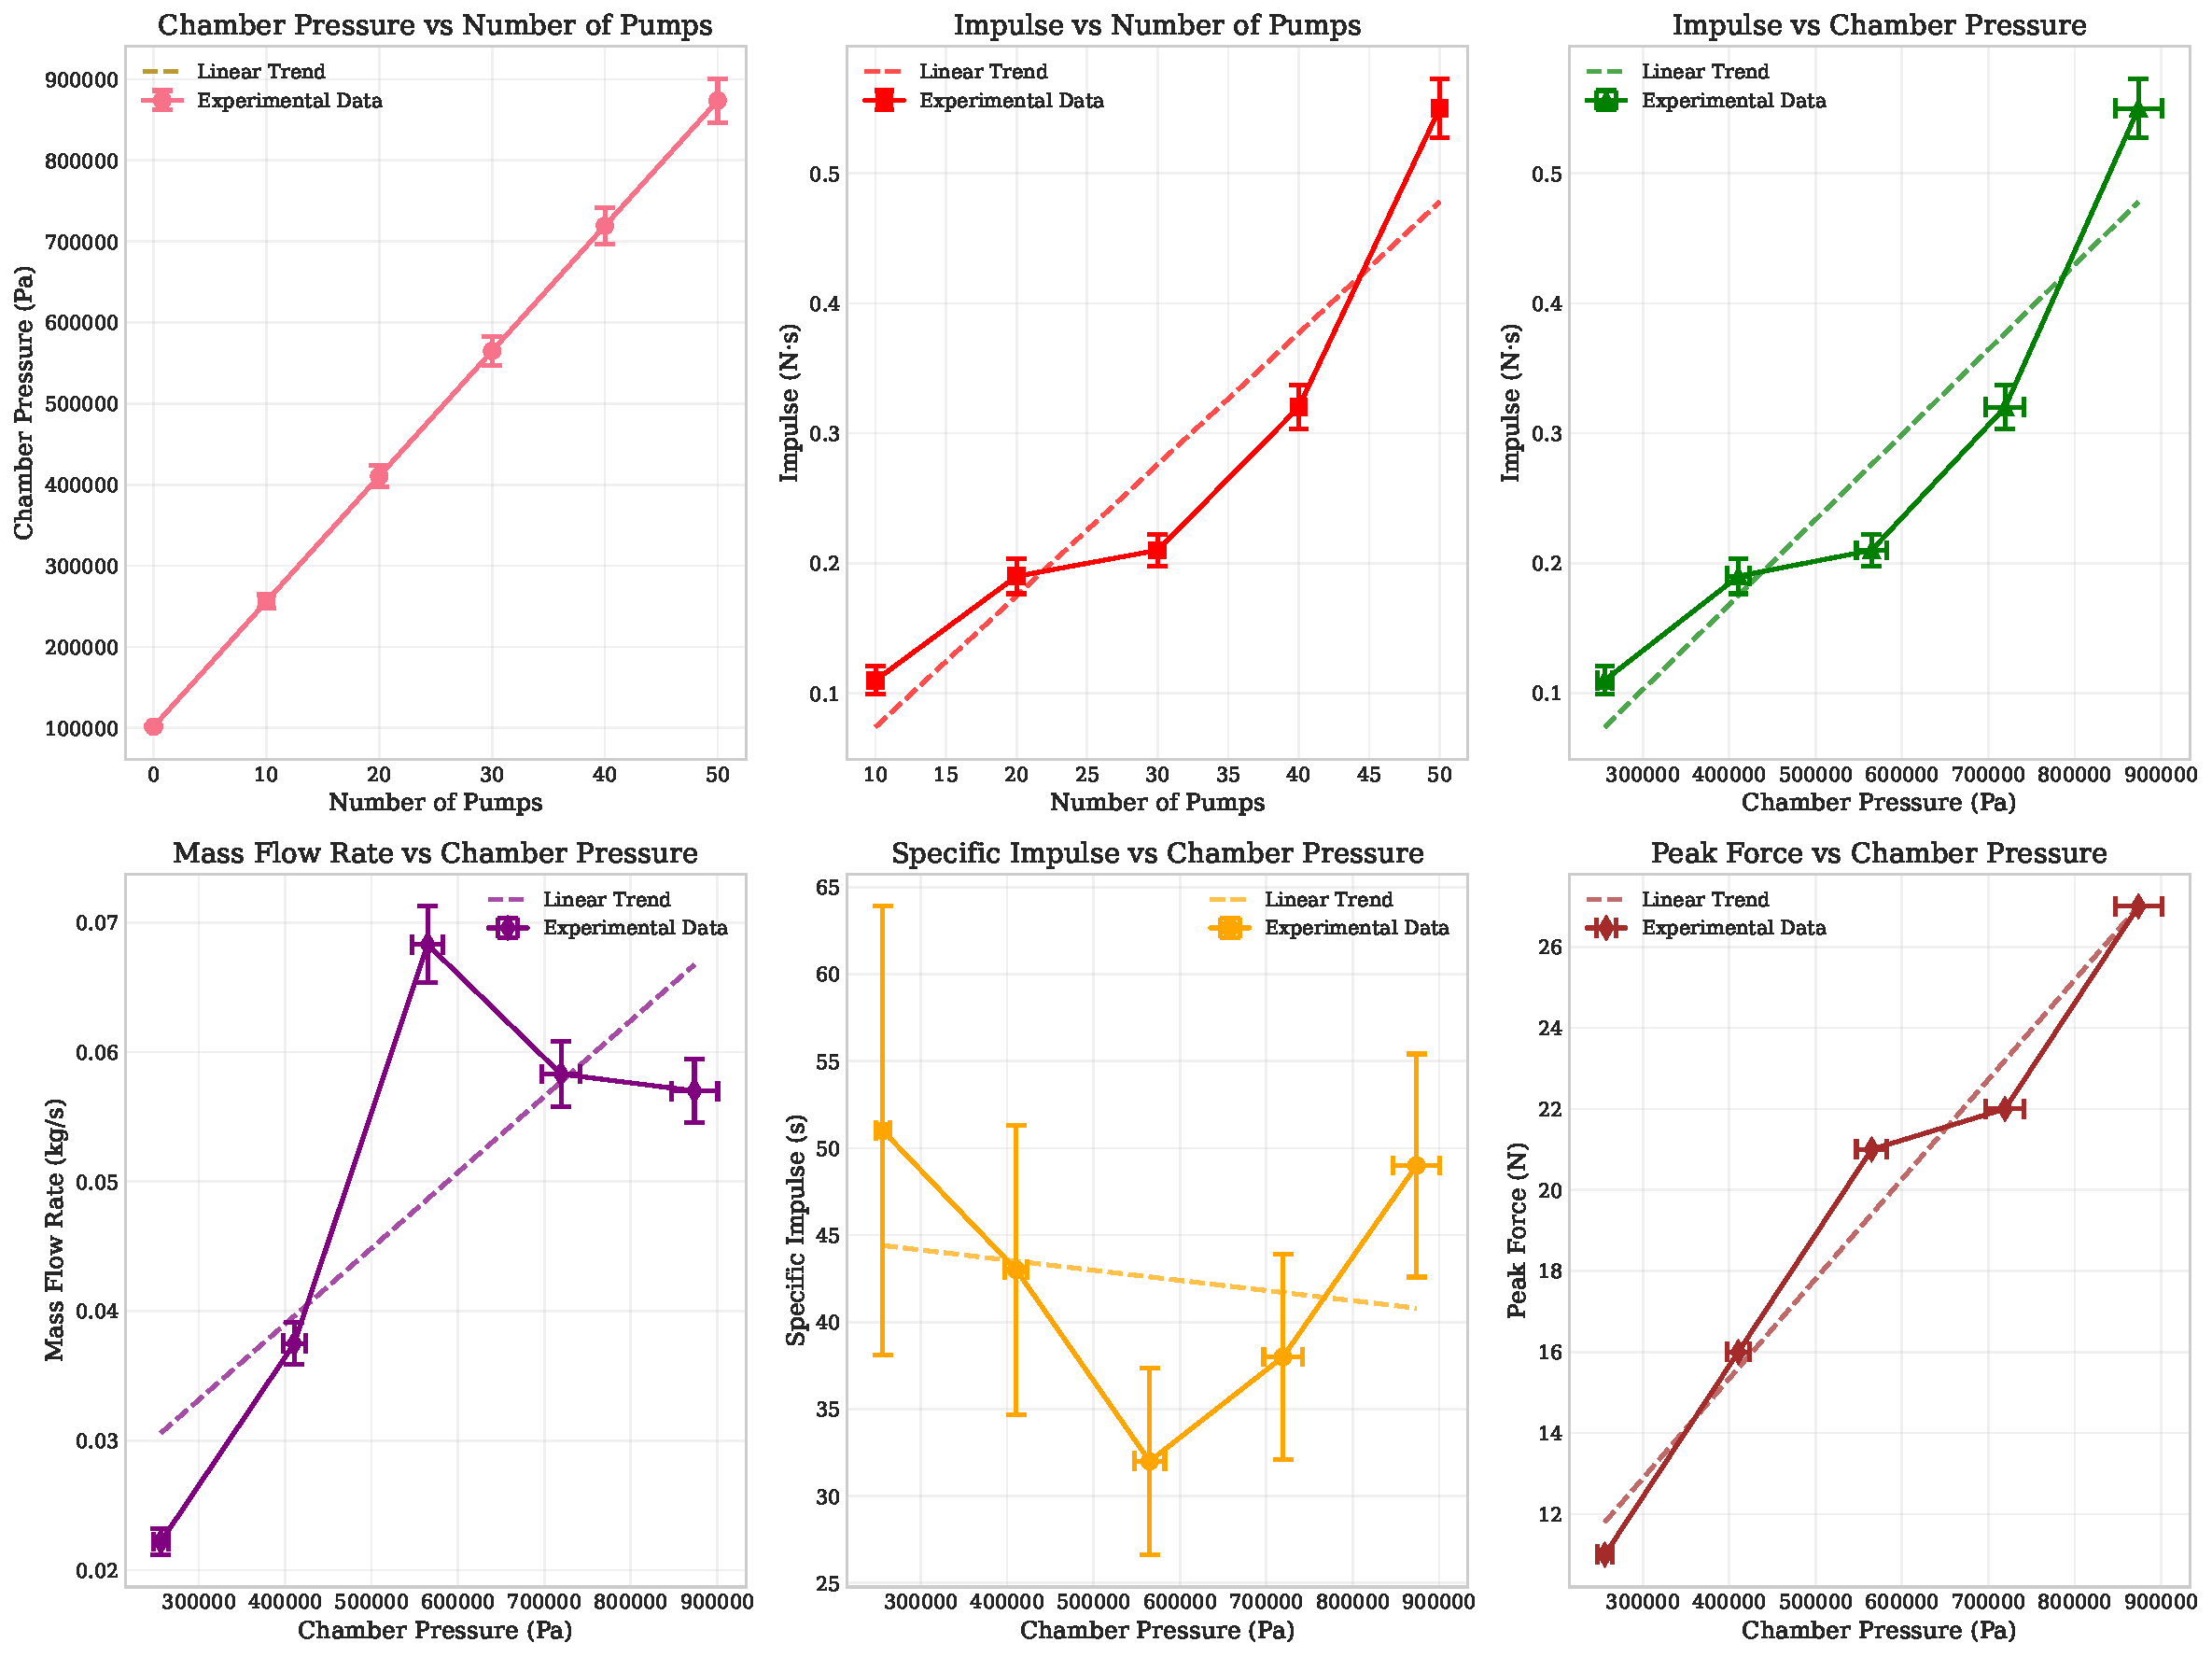
\includegraphics[width=0.9\textwidth]{physics_ia_comprehensive_analysis.pdf}
 \caption{in these graphs i have left in pumps as a independent variable, to show that there is the same correlation nomatter in what unit pressure is reprecentet, seen here are all corelation measured.}
\label{fig:comprehensive_analysis}
\end{figure}

\begin{figure}[H]
\centering
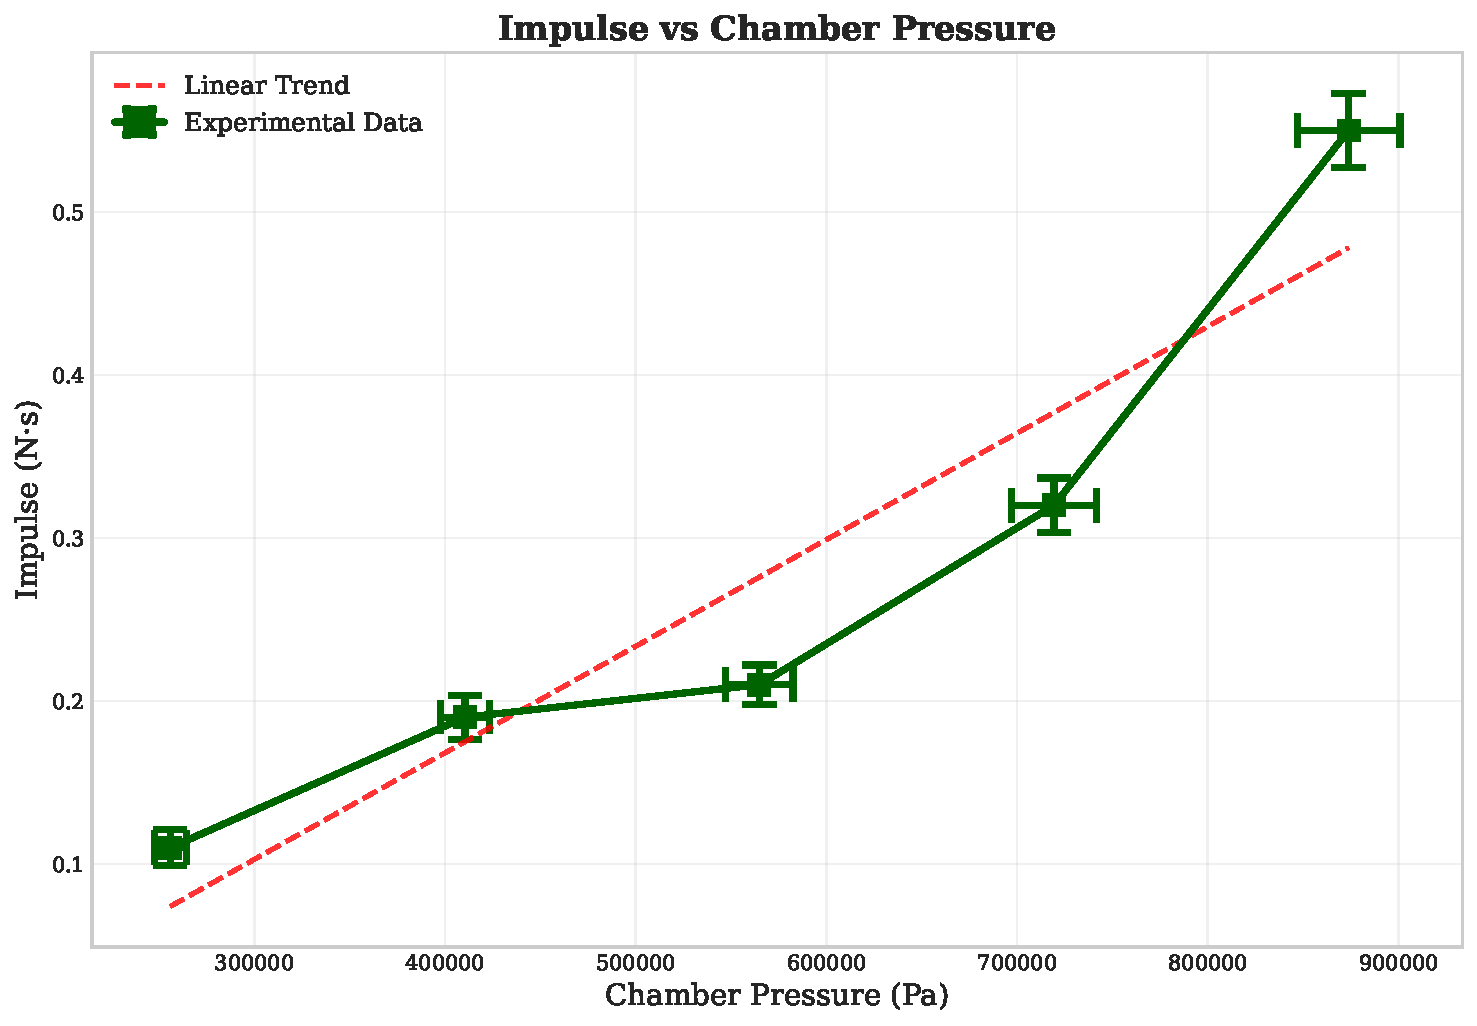
\includegraphics[width=0.9\textwidth]{impulse_vs_pressure.pdf}
    \caption{this graph shows impulse as a funciton of pressure, bigger for better visualization}
\label{fig:impulse_pressure}
\end{figure}

\begin{figure}[H]
\centering
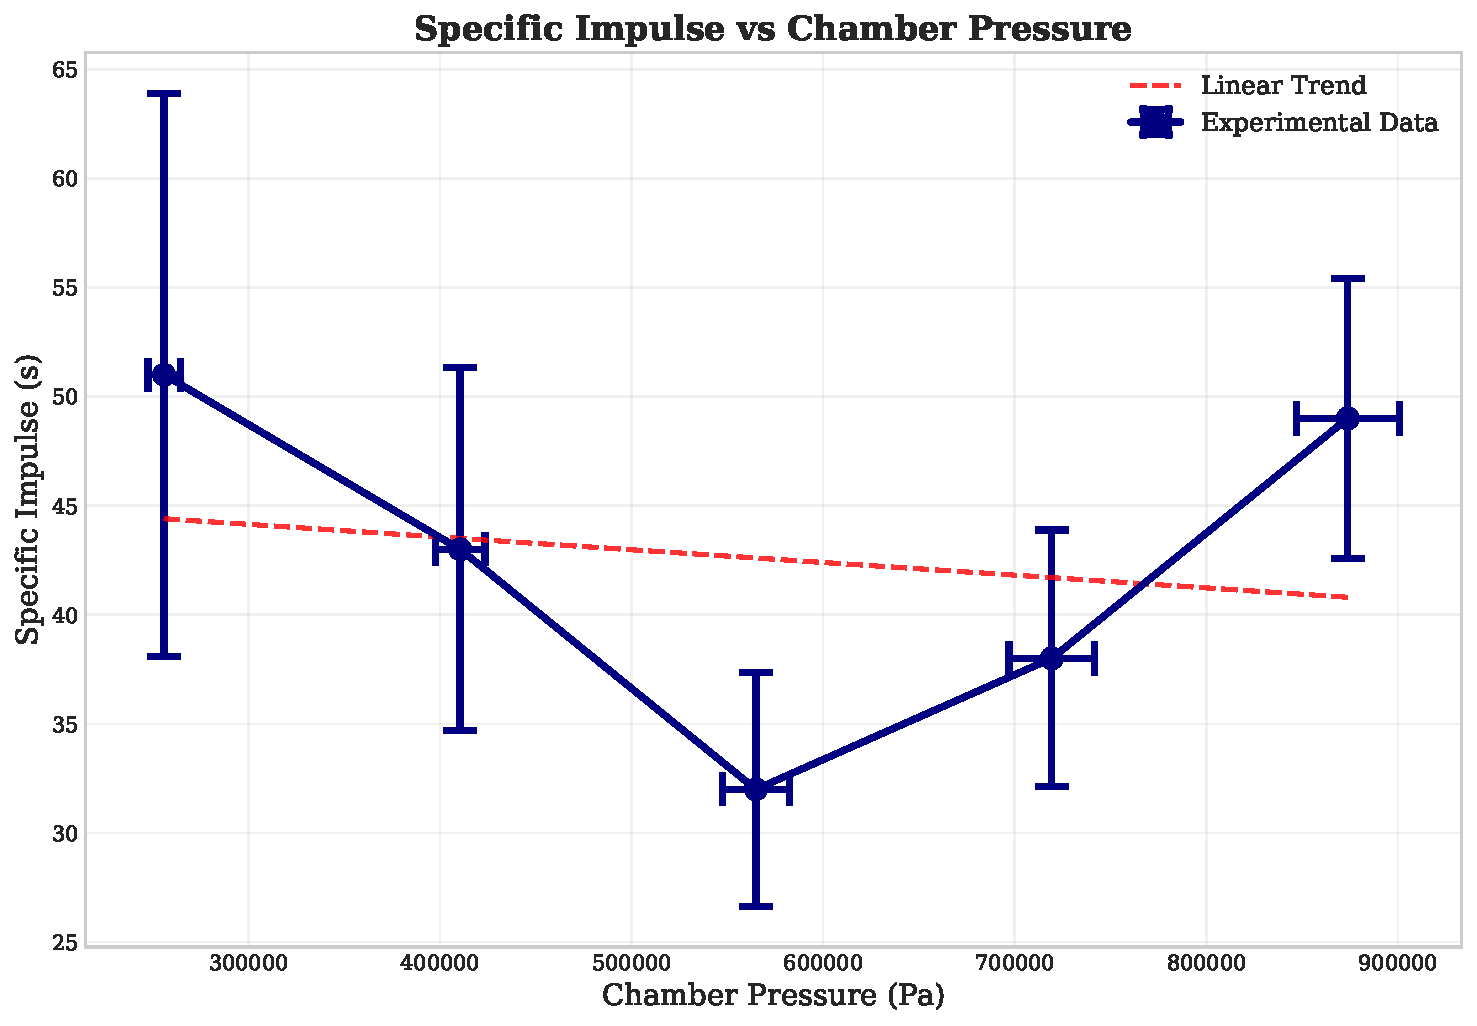
\includegraphics[width=0.9\textwidth]{specific_impulse_vs_pressure.pdf}
\caption{this graph shows specific impulse as a fuction of pressure,  bigger for better visualization}
\label{fig:specific_impulse_pressure}
\end{figure}

\section{Data Analysis}

\subsection{Processing the Data}

I had an incredible increase and range in pressure which I didn't actually expect, reaching all the way to more than 8 times atmospheric pressure. It would seem that one expects this to have a significant impact on performance. Then unfortunately there seems to be an outlier, 30 pump measuring point, which is constantly deviating from the other expected values.

I think this might be because after finding leaks in my palimetery i added more o rings to seal the chamber, it could be that even those rings did not seal the chamber correctly after pressures exceeded the pressure at 30 pumps reducing the actual pressure in the chamber than what i calculated due to leaks, for the following measurements. But I did not witness any signs of leaks when conducting my experiment.

\subsection{Interpretation of Graphs}

From looking at the graphs it is obvious that an increase in pressure very much increases impulse very directly, with a strong correlation, both against number of pumps and pressure. The correlation between pressure and mass flow rate is almost as strong, but the angle of the line is less steep, this is probably because the nozzle throat does not limit the amount of mass that can exist at a time, which means the time which it takes for the mass to flow out is longer because there is more air particles in the rocket and therefore mass flow is strongly affected. And because the mass flow rate seems to be affected in this way the higher force measured gets cancelled out in the formula for specific impulse where we divide by the mass flow rate. In turn the higher force gets divided by a higher mass flow rate dampening the change, due to pressure. Resulting in the bad correlation between pressure and specific impulse.

Which is actually interesting to find out as well, I did not consider that both changes can cancel each other out leading to almost no visible correlation between pressure and specific impulse.

Although it has to be said that the uncertainty of 25\% could also mean that the correlation might not be visible even though there may actually be one.

\section{Evaluation}

\subsection{Strengths and Weaknesses}

I think my experiment overall was not too bad, I did not go into this experiment expecting a crazy correlation so I am very happy with my findings. Apart from my force uncertainties which i was unable to impact as i had one force plate as an option only, i think that especially my uncertainties which i made sure to keep low after preliminary testing were very strong.

A big weakness though was probably the noise and inconsistency of my readings. The force plate was constantly measuring force changes, only $\pm$ \SI{1}{\newton}, even if nothing was happening, this created some noise in my data which was hard to account for, and possibly my data would have been different. Also the inconsistency of my force and time measurements were not good, the spread across my measurements were too big for my likings.

Even Though i very much enjoyed calculating surrounding variables like the pressures and the density of air, I think there might be better solutions possible. But actually it doesn't matter what the actual values are for this experiment as I am only investigating the correlation, and that would stay the same no matter if the values were wrong.

\subsection{Sources of Error}

A big source of my force readings will likely be that the force plate used was designed for far bigger forces which affect its accuracy and the accuracy of my measurements in the experiment.

Not having equipment that can measure ambient pressure or that can take tests on the surrounding air, might have caused any wrong calculations due to researched values.

\subsection{Improvements}

Next time I would possibly look into using a scale as a force plate instead, which often goes to 0.001 gramms significant figures, far more accurate then the force plate, and then accounting for gravity to calculate the forces. This could decrease the \%uncertainty and reduce the inconsistency of measurements.

Getting access to measurement equipment which can measure more atmosphere specific things similar to once used in weather stations could have a huge impact on the relevance of my measurements to the surroundings of my experiment.

After digging even deeper I found that the mass flow rate is changing differently in proportion to pressure after the gases reach mach 1 in the engine, because of the shock created in the nozzle limiting the mass flow rate completely, choking it, any further increase in pressure does not contribute to increase in mass flow rate. It is very possible that my experiment never choked at the nozzle, which means that there is a possibility for a stronger correlation from pressure to specific impulse at even higher pressures. So for future experiments, investigating how specific impulse is affected by pressure at high speed nozzles like the bell nozzle can be interesting as well, or at even higher pressures like my references like 100 bar.

Also using a proper converging diverging nozzle could lead to higher exhaust speeds, instead of just using a small hole. I have not listed this in sources of error, because the measurements would not be affected, the nozzle is constant throughout the measurements. But higher exhaust speed can contribute to the choked nozzle, giving the same possibility for a higher correlation between pressure and specific impulse.

Considering that one of my errors might be caused due to leaks as mentioned as a outlier. in the future, I would like to experiment with a correctly sealed real rocket engine, assuming that this can survive even higher pressures and does not leak.

\section{Conclusion}

In conclusion the chamber pressure of a rocket could have some impact on the specific impulse, and being able to reach higher pressures inside a rocket can be beneficial, as long as it is safe. But there might be other variables to look into which affect specific impulse more strongly.

From this research I will be able to use my understanding to go out and design my rocket engine to be able to withstand higher pressures, although all pressures used in this experiment were only close to 8 bars I am looking forward to predicting even higher specific impulse in my rocket at 100-200 bars.

\section{Appendix}

Here we can see how i conducted the experiment:

\begin{figure}[H]
\centering
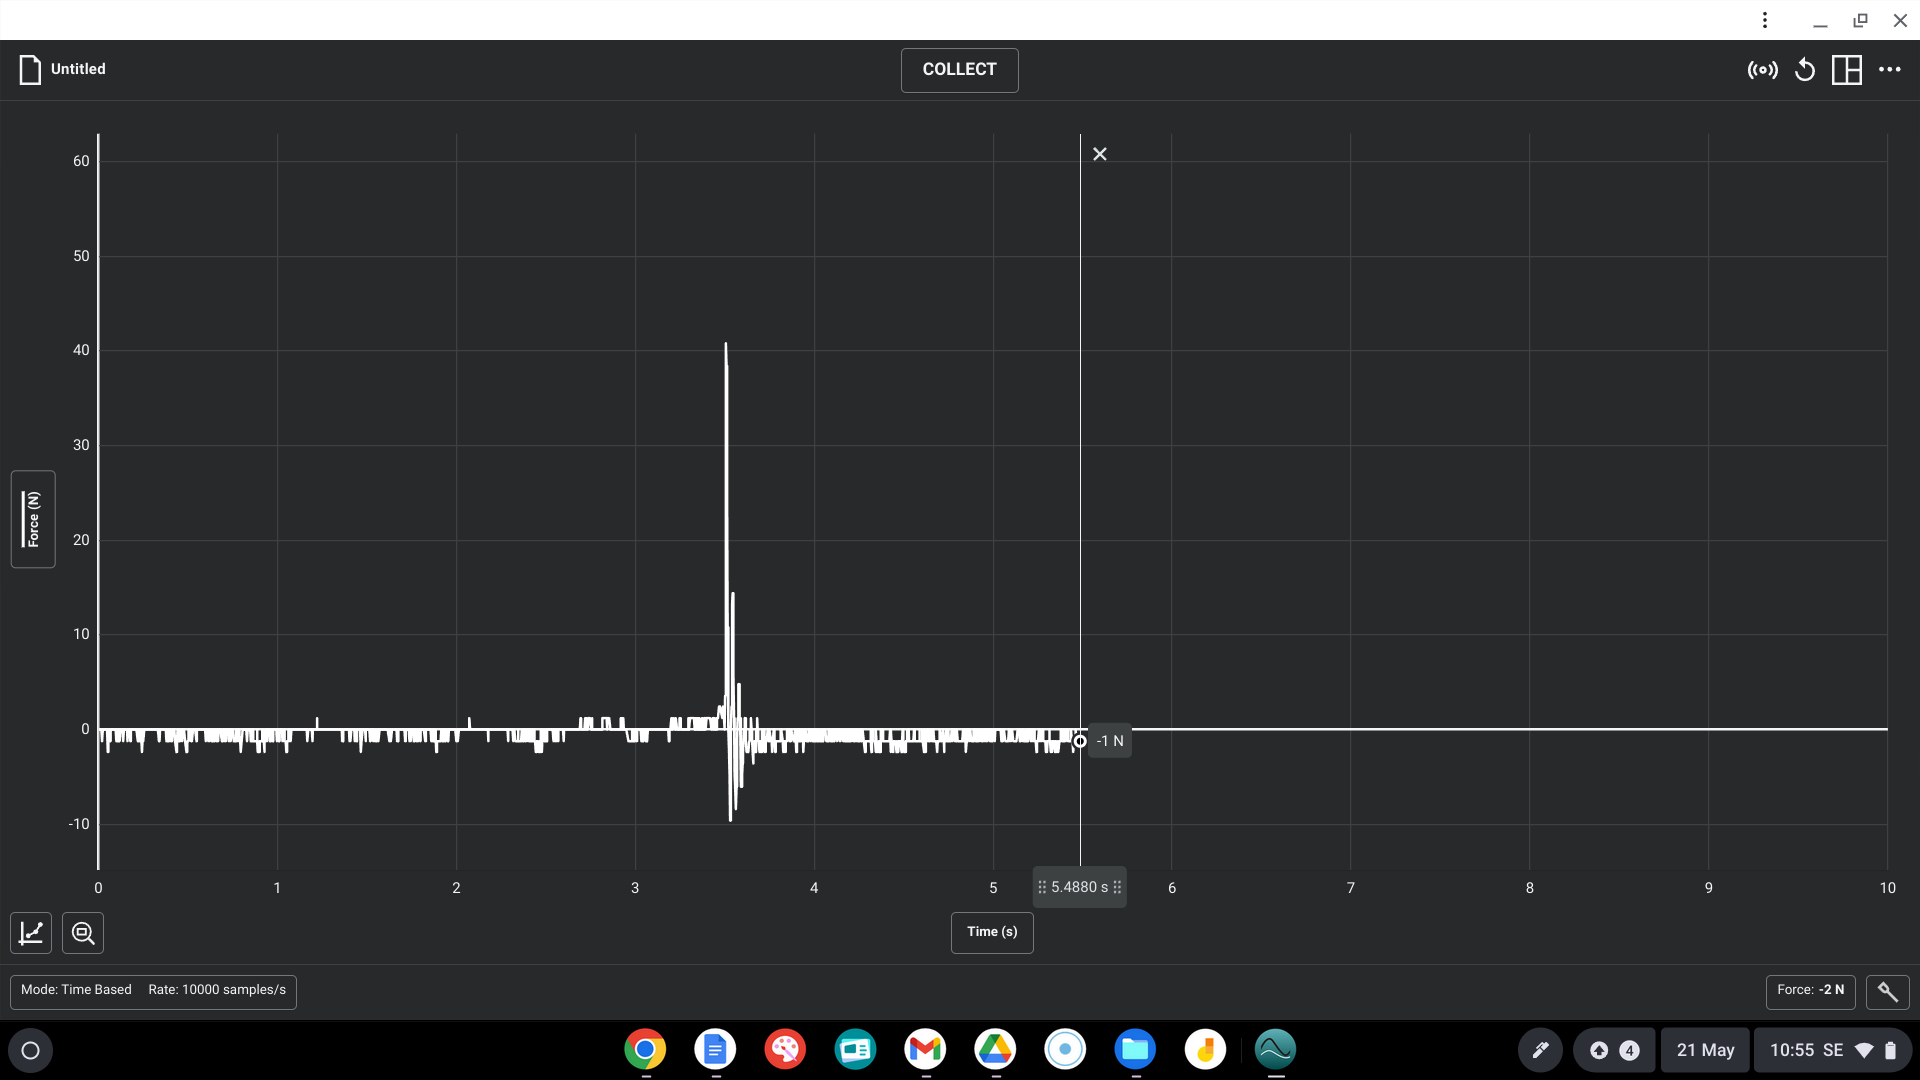
\includegraphics[width=0.8\textwidth]{measering apendix.png}
\caption{Measurement appendix}
\label{fig:measurement_appendix}
\end{figure}

\begin{figure}[H]
\centering
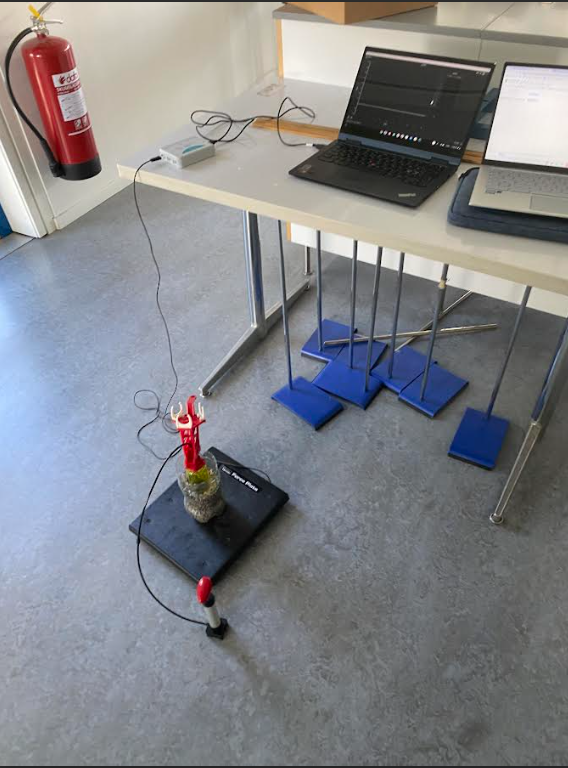
\includegraphics[width=0.8\textwidth]{measuring data appendix.png}
\caption{Measuring data appendix}
\label{fig:data_appendix}
\end{figure}

\begin{figure}[H]
\centering
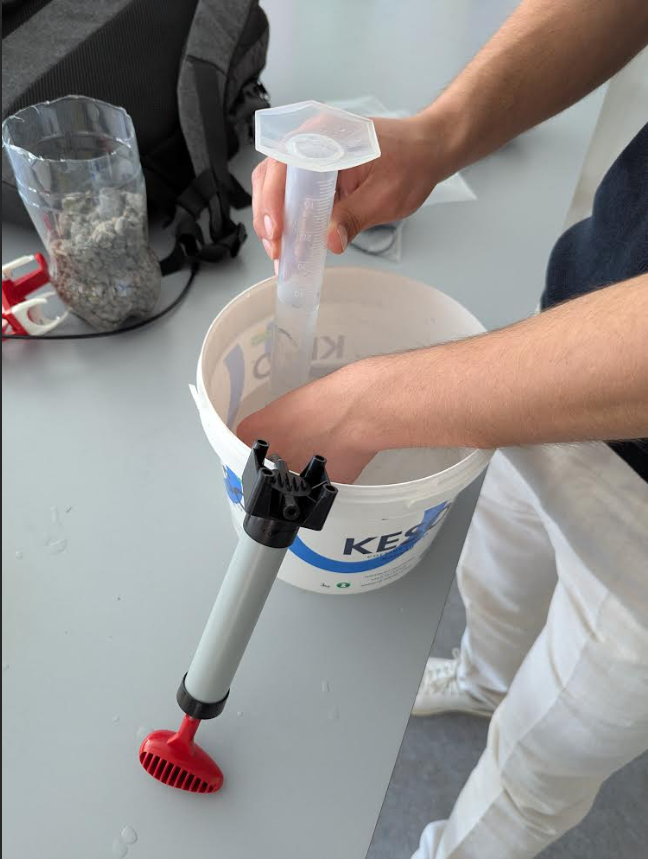
\includegraphics[width=0.8\textwidth]{measuring water sicplacment appendix.png}
\caption{Measuring water displacement appendix}
\label{fig:water_displacement_appendix}
\end{figure}
atmospheric pressure, from weather app:
\begin{thebibliography}{99}

\bibitem{ref1}
How is chamber pressure determined for rocket engines? \url{https://space.stackexchange.com/questions/21758/how-is-chamber-pressure-determined-for-rocket-engines}

\bibitem{ref2}
Chamber pressure research. \url{https://lup.lub.lu.se/luur/download?func=downloadFile&recordOId=9183792&fileOId=9183793}

\bibitem{ref3}
Rocket Propulsion. \url{https://phys.libretexts.org/Bookshelves/University_Physics/University_Physics_(OpenStax)/Book:_University_Physics_I_-_Mechanics_Sound_Oscillations_and_Waves_(OpenStax)/09:_Linear_Momentum_and_Collisions/9.11:_Rocket_Propulsion}

\bibitem{ref4}
Rocket Propulsion. \url{https://pressbooks.online.ucf.edu/osuniversityphysics/chapter/9-7-rocket-propulsion/}

\bibitem{ref5}
Rocket Propulsion. \url{https://web.mit.edu/16.unified/www/SPRING/propulsion/notes/node103.html}

\bibitem{ref6}
Mass Flow Rate. \url{https://engineerexcel.com/mass-flow-rate/}

\bibitem{ref7}
Mass flow rate research. \url{https://www.mdpi.com/1996-1073/17/24/6455}

\bibitem{ref8}
What is Specific Impulse? \url{https://web.archive.org/web/20160704233223/http://www.qrg.northwestern.edu/projects/vss/docs/Propulsion/3-what-is-specific-impulse.html}

\bibitem{ref9}
Specific Impulse. \url{https://www.grc.nasa.gov/WWW/k-12/airplane/specimp.html}

\bibitem{ref10}
Nozzle Design. \url{https://web.archive.org/web/20060825031851/http://trs.nis.nasa.gov/archive/00000186/01/sp8120.pdf}

\bibitem{ref11}
Nozzle Design. \url{https://wikis.mit.edu/confluence/pages/viewpage.action?pageId=153816550}

\bibitem{ref12}
Rocket Engines. \url{https://eaglepubs.erau.edu/introductiontoaerospaceflightvehicles/chapter/rocket-engines/}

\bibitem{ref13}
Fuel Efficiency in Spacecraft. \url{https://spacevoyageventures.com/fuel-efficiency-in-spacecraft-innovations-in-propulsion-and-energy-use/}

\bibitem{ref14}
Density of air. https://srjcstaff.santarosa.edu/~oraola/CHEM1ALECT/Ch.%2005/waals.pdf

\bibitem{ref15}
Local gravity. https://bgi.obs-mip.fr/data-products/gravity-databases/land-gravity-data-prod/#/data/land

\end{thebibliography}

\end{document}
